\documentclass[10pt]{article}
\usepackage{tikz}
\usetikzlibrary{shapes.geometric, arrows}
\usetikzlibrary{positioning}
\usepackage[most]{tcolorbox}
\usepackage{hyperref}
\usepackage{geometry} 
\usepackage{xpatch}
\usepackage{xcolor}
\usepackage{listings}
\usepackage{realboxes}
\usepackage{subfig}
\usepackage{float}
\geometry{a4paper, left=10mm, right=10mm, top=20mm} 

% Set TikZ styles
\tikzstyle{arrow} = [thick,->,>=stealth]
\tikzstyle{doublearrow} = [thick,<->,>=stealth]
\tikzstyle{startstop} = [rectangle, rounded corners, minimum width=3cm, minimum height=1cm,text centered, draw=black, fill=red!30]
\tikzstyle{io} = [trapezium, trapezium left angle=70, trapezium right angle=110, minimum width=3cm, minimum height=1cm, text centered, draw=black, fill=blue!30]
\tikzstyle{process} = [rectangle, minimum width=3cm, minimum height=1cm, text centered, draw=black, fill=orange!30]
\tikzstyle{decision} = [diamond, minimum width=3cm, minimum height=1cm, text centered]

% Do not indent first line of new paragraphs not following sections
\setlength\parindent{0pt}

% \usepackage{amsmath} % \usepackage is a command that allows you to add functionality to your LaTeX code
\usepackage{titling}
\usepackage{graphicx} % the demo option is just for the example

\graphicspath{ {.././images/} } % Where to find images

% Set inline code style
\definecolor{code_background_color}{rgb}{0.8,0.8,0.8}
\lstset{
  basicstyle=\ttfamily,
  backgroundcolor=\color{code_background_color},
}

\makeatletter
\xpretocmd\lstinline{\Colorbox{code_background_color}\bgroup\appto\lst@DeInit{\egroup}}{}{}
\makeatother

% Setup document link styles
\hypersetup{
    colorlinks,
    citecolor=black,
    filecolor=black,
    linkcolor=blue,
    urlcolor=blue
}

%textmarker style from colorbox doc
\tcbset{textmarker/.style={%
        enhanced,
        parbox=false,boxrule=0mm,boxsep=0mm,arc=0mm,
        outer arc=0mm,left=6mm,right=3mm,top=7pt,bottom=7pt,
        toptitle=1mm,bottomtitle=1mm,oversize}}


% define new colorboxes
\newtcolorbox{hintBox}{textmarker,
    borderline west={6pt}{0pt}{yellow},
    colback=yellow!10!white}
\newtcolorbox{importantBox}{textmarker,
    borderline west={6pt}{0pt}{red},
    colback=red!10!white}
\newtcolorbox{noteBox}{textmarker,
    borderline west={6pt}{0pt}{green},
    colback=green!10!white}
\newtcolorbox{infoBox}{textmarker,
    borderline west={6pt}{0pt}{blue},
    colback=blue!10!white}
  

% define commands for easy access
\newcommand{\info}[1]{\begin{infoBox} \textbf{Info:} #1 \end{infoBox}}
\newcommand{\note}[1]{\begin{noteBox} \textbf{Note:} #1 \end{noteBox}}
\newcommand{\warning}[1]{\begin{hintBox} \textbf{Warning:} #1 \end{hintBox}}
\newcommand{\important}[1]{\begin{importantBox} \textbf{Important:} #1 \end{importantBox}}

% Show NSPanelManager logo on first page above title
\pretitle{%
  \begin{center}
  \LARGE
  
\includegraphics{logo.png}\\[\bigskipamount]
}
\posttitle{\end{center}}

\title{User \& Technical reference manual} % Sets article title
\author{} % Sets authors name
\date{} % Sets date for date compiled

% The preamble ends with the command \begin{document}
\begin{document} % All begin commands must be paired with an end command somewhere
    \maketitle % creates title using information in preamble (title, author, date)

    \clearpage
    \tableofcontents
    \clearpage
    \section{Introduction} % creates a section
    NSPanel Manager is a custom software solution for the Sonoff NSPanel (not the NSPanel pro). The software is designed to be easy to use on a day to day basis and to easily manage multiple NSPanels around your home.
    The interface on the NSPanel itself has been designed to be intuitive to use for people of all ages and backgrounds.
    \bigbreak
    All the NSPanel that are installed with the NSPanel Manager solution communicate back to a Docker container that is used to manage the panels, NSPanel Manager specific solutions and also all communication back and forth to/from Home Assisant and/or OpenHAB.

    \clearpage
    \section{Quick start guide}
    \subsection{Container setup}
    Prerequisites:
    \begin{itemize}
      \item Repository cloned/downloaded.
      \item Working Docker installation.
    \end{itemize}
    \subsubsection{Standalone Docker container}
    At the moment, the container image is not available on any registry. This means that the image has to be built manually to start it. If running MacOS or Linux this is easy enough to do, perform the following to build and start the container:
    \begin{itemize}
      \item Open a terminal and navigate to the downloaded repository.
      \item Execute \lstinline[language=bash]|cd docker| to navigate to the "docker"-directory.
      \item Run the script "docker-build\_and\_run.sh" to build the container \& start it up using the default values. This can be done by executing \lstinline[language=bash]|bash docker-build_and_run.sh|.
    \end{itemize}
    If you wish to manually build and run the container, see below for \hyperref[sec:advanced_setup]{advanced setup}.

    \subsubsection{Home Assistant add-on}
    As the repository is set to private currently, there is no way of adding it as a repository to Home Assistant. This can be worked around by doing the following:
    \begin{itemize}
      \item In Home Assistant, install the Samba or SSH add-on.
      \item Access the "addons"-directory in Home Assistant and create a new directory called "nspanelmanager".
      \item Copy all the files in the "docker"-directory from the GitHub repository to the newly created "nspanelmanager"-directory on the Home Assistant machine.
      \item In the Home Assistant web interface, navigate to Settings -> Add-ons -> Add-on store.
      \item In the upper right corner, press the three dots and choose "Check for updates".In a few seconds the "NSPanel Manager" add-on should show up under "Local add-ons".
      \note{If the add-on has not appeared within 30 seconds, try refreshing the page and trying again.}
      \note{Some users have reported that Home Assistant has to be restarted for it to show the new add-on.}
      \item Select the "NSPanel Manager" add-on and install it.
      \item Check that the add-on should start automatically.
      \item Start the add-on.
    \end{itemize}
    \subsection{Container settings}
    The following has to be done in order to get a fully working container:
    \begin{itemize}
      \item Navigate to the web interface. If the port was not changed it is available at port \textbf{8000}.
      \item Enter MQTT server.
        \note{If you are running the MQTT server as an add-on to Home Assistant, enter the IP-address of your Home Assistant server.}
      \item Enter MQTT port if changed from default \textbf{1883}.
      \item If authentication is used for MQTT, enter username and password.
      \item If running Home Assistant, enter address with http or https and port, Ex. \textit{http://192.168.1.5:8123}. Also enter Home Assistant access token.
      \info{To get an access token in Home Assistant, navigate to Home Assistant and press your username in the bottom left. Scroll down and create a "Long-Lived Access Token".}
      \info{If you are running the container as an Home Assistant add-on, the address and access token will already be set. Do not change these.}
      \item If running OpenHAB, enter address with http or https and port, Ex. \textit{http://192.168.1.5:8080}. Also enter OpenHAB access token.
      \info{To get an access token in OpenHAB, navigate to OpenHAB and press your username in the bottom left. Scroll down and create an "API Token".}
    \item Save the new settings and continue to \hyperref[sec:nspanel_flashing]{NSPanel flashing}.
    \end{itemize}

    \subsection{NSPanel flashing}
    \label{sec:nspanel_flashing}
    Prerequisites:
    \begin{itemize}
      \item Working TTL flasher for 3.3V.
      \item Working serial setup for your PC and known serial port (in Windows known as COM-port).
    \end{itemize}
    In order to connect to the NSPanel and be able to flash it, you must dismantle it. For a guide on how to dismantle and connect your serial flasher to the NSPAnel, refer to \href{https://www.youtube.com/watch?v=p-AK4o5jOSI}{this} guide from MarkWattTech.
    \subsubsection{Flashing with Espressif ESP32 DOWNLOADER TOOL (Windows only)}
    To flash the panel, perform the following:
    \begin{itemize}
      \item Download the tool from Espressif from \href{https://www.espressif.com/en/support/download/other-tools}{here}.
      \item Open the tool and choose to flash an ESP32 chip.
      \item Check one checkbox and select the "merged\_flash.bin"-file in the "docker/web/nspanelmanager/"-directory.
      \item Enter "0x0" as the upload address.
      \item Connect your flasher to the NSPanel and press "START".
    \end{itemize}
    \begin{center}
    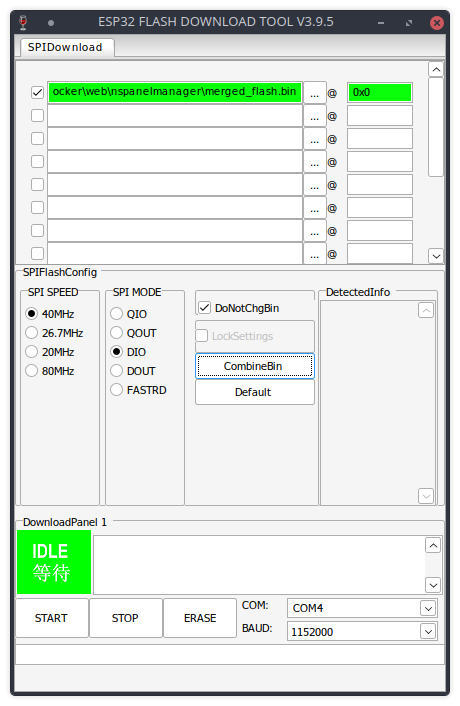
\includegraphics[scale=0.4]{esp_flash_download_tool.png}
    \end{center}
    \subsubsection{Flashing with ESPtool (all operating systems)}
    By installing esptool it is possible to upload the merged flash using the command line. Do the following:
    \begin{itemize}
      \item Open a terminal.
      \item Navigate to the "docker/web/nspanelmanager/"-directory.
      \item To determine if you have selected the right port, run \lstinline[language=bash]|esptool.py flash_id --port <port>|. You will have to replace "<port>" with the actual port connected to the NSPanel. This will do a check and see if the tool can communicate with the NSPanel.
      \item Run \lstinline[language=bash]|esptool.py --baud 921600 --port /dev/ttyUSB0 write_flash 0x0 merged-flash.bin|. You will have to replace "/dev/ttyUSB0" with the actual port connected to the NSPanel.
      \info{On Windows it might be just "esptool" without the ".py" at the end.}
      \info{On Windows "/dev/ttyUSB0" will have to be replaced by something like "COM4". If using MacOS or Linux the port will be something similar to "/dev/ttyUSB0".}
    \end{itemize}
    After the flashing is complete you can continue with \hyperref[sec:nspanel_configuration]{NSPanel configuration}.
 
    \subsection{NSPanel configuration}
    \label{sec:nspanel_configuration}
    To configure the NSPanel, do the following:
    \begin{itemize}
      \item Power up the panel.
      \warning{If you have flashed multiple NSPanels, power them up one at a time as they will all have the same WiFi access point name.}
      \info{The GUI file has not been flashed yet so there will not be any visible change on the NSPanel screen.}
      \item Connect to the new WiFi network "NSPMPanel" when the panel has started.
      \item When connected to the new WiFi network, make sure your device does not disconnect because it detects no internet access. Then open a browser and navigate to "http://192.168.1.1".
      \info{There have been issues when using Android and the Chrome browser that it sometimes just shows a blank page. If this is the case, either use a different browser (Ex. Firefox) or another device with WiFi to access the web page.}
      \item Enter a friendly name for the NSpanel.
      \note{This name is only used to register the NSPanel the first time. After the panel has been registered the name can be changed from the manager web interface.}
      \item Enter the IP-address for the manager docker container.
      \item Enter the port for the manager if changed during container setup.
      \item Enter WiFi name and password.
      \item Enter MQTT address and port.
      \note{If you are running the MQTT server as an add-on to Home Assistant, enter the IP-address of your Home Assistant server.}
      \item Press the "Save" button on the bottom of the page. The panel will reboot and try to connect to the WiFi network.
      \info{If the panel fails to connect to the WiFi network for three minutes it will revert back and start the access point again. It will periodically scan for the configured WiFi and, if it detetacts that the configured WiFi has come back, it will reboot and connect to it.}
      \item Connect to your WiFi again and go to the NSPanel Manager web interface. If all things are working and setup correctly the panel should show up in the list of panels on the first page.
      \info{If this is a US NSPanel version then it has to be set in the panel settings. Press the name of the NSPanel in the list and check the "Is US panel"-checkbox.}
      \item Flash the new GUI file to the panel by pressing the "Actions"-button on the right and select "Update screen".
      \note{The flashing of the GUI file may be finicky and might require multiple tries before it succeeds. If it fails and reboots or you see a "System data error", just try again.}
    \end{itemize}

    \section{NSPanel Manager web interface}
    The web interface is partitioned into 4 main sections.
    \begin{enumerate}
      \item The first page where panel status and management can be done.
      \item The panel settings page.
      \item The Room page.
      \item The global settings.
    \end{enumerate}
    Below, each section of the web interface is described.
    \subsection{First page}
    The first page is used to get an overview of each registerd NSPanel as well as perform actions on each panel. These actions are:
    \begin{itemize}
      \item Reboot.
      \item Firmware update.
      \item GUI update.
      \item Delete.
    \end{itemize}
    By pressing the name of the NSPanel you will get to the \hyperref[sec:nspanel_page]{NSPanel settings page}. By pressing the room name you will get to the relevant \hyperref[sec:room_page]{room settings page}. By pressing the IP-address of the panel a new tab will open with the configuration page on the actual NSPanel.
    \\
    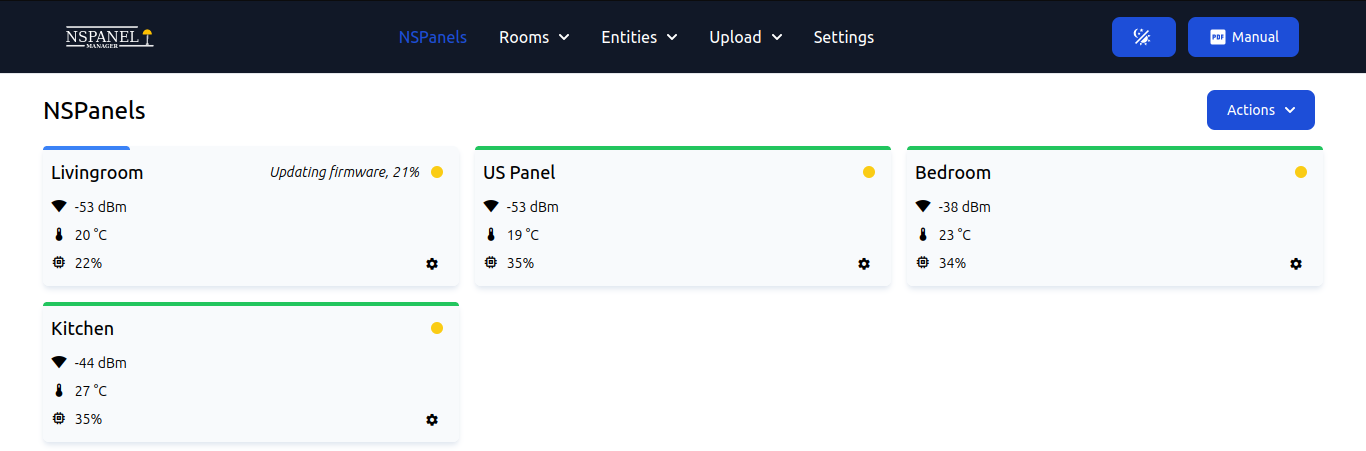
\includegraphics[width=\textwidth,height=\textheight,keepaspectratio]{index_page.png}
    \subsection{NSPanel page}
    \label{sec:nspanel_page}
    On the NSPanel settings page, settings specific for one NSPanel can be made. This is things like name, default room and so on. There is also a live display of any log messages sent from the chosen NSPanel. This depends on the selected log level in the NSPanel configuration page which is available at the IP address of the NSPanel itself.
    \\
    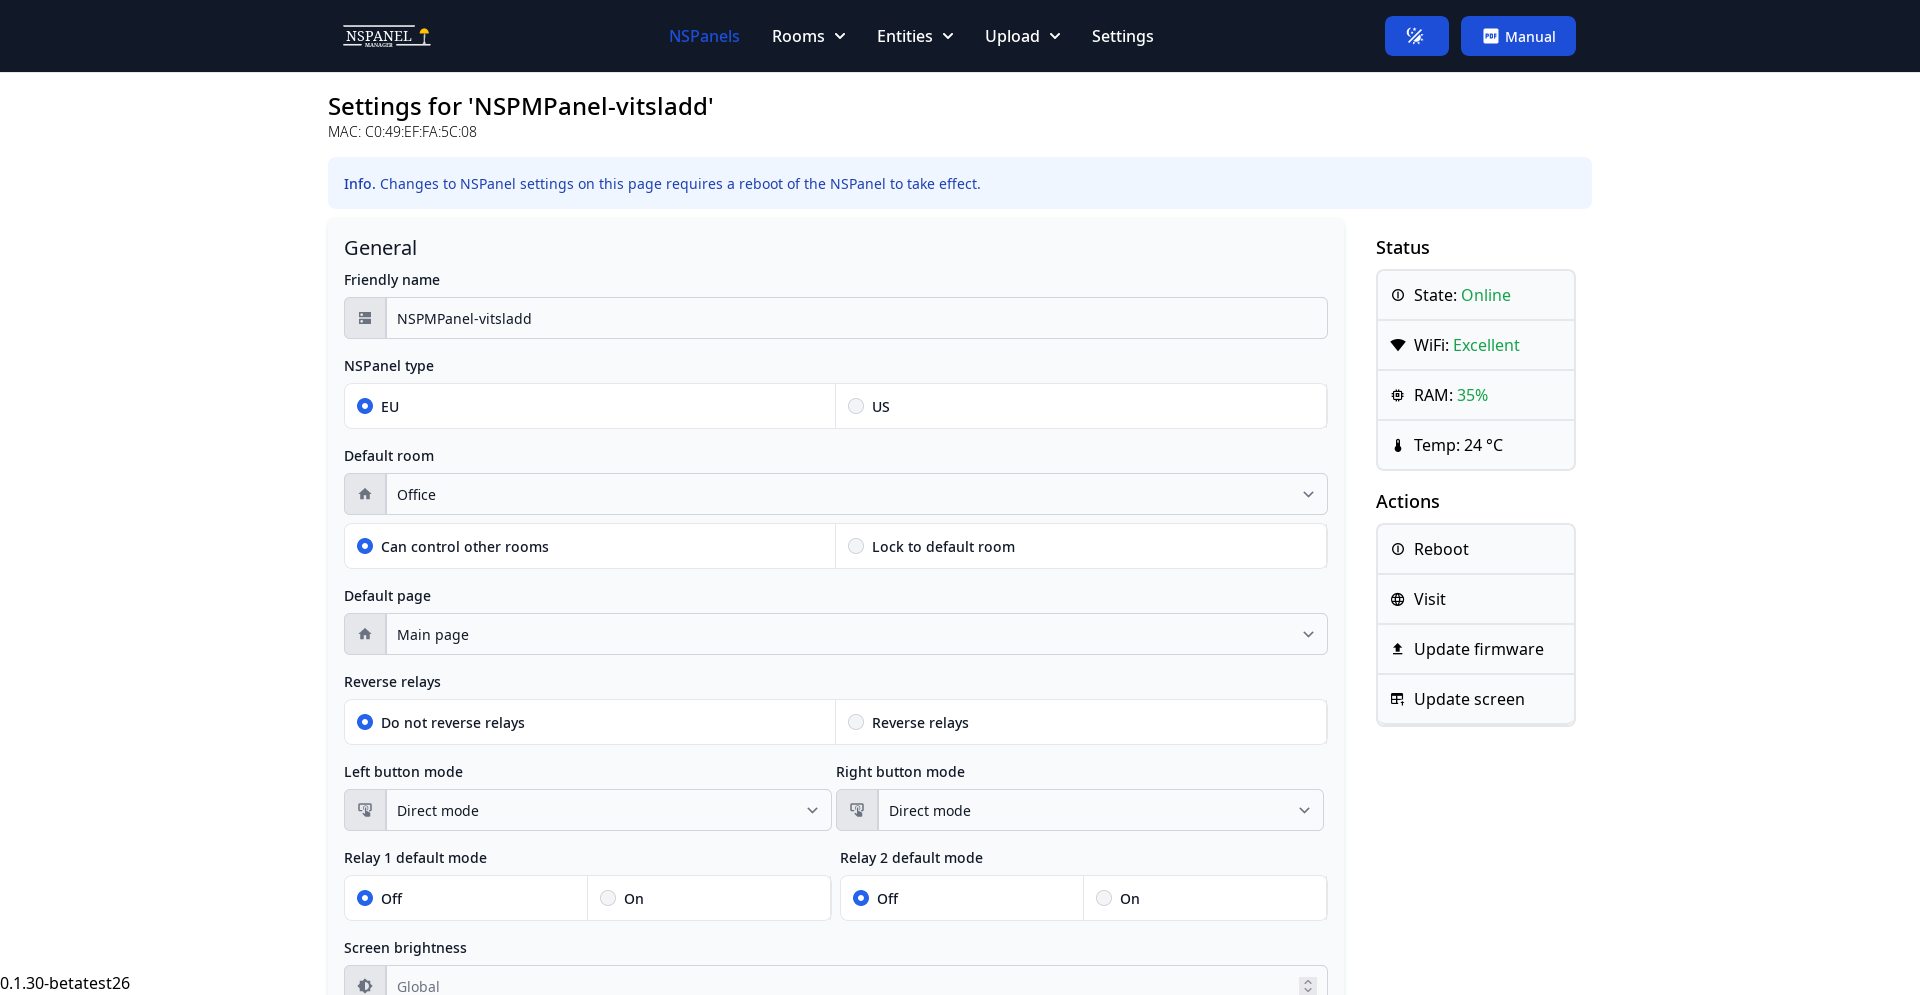
\includegraphics[width=\textwidth,height=\textheight,keepaspectratio]{nspanel_page.png}
    \subsection{Room page}
    \label{sec:room_page}
    This section will describe how to manage rooms. Most of the configuration done with NSPanel Manager will be done in rooms, please read this chapter for a full understanding on how to work with rooms.
    \\
    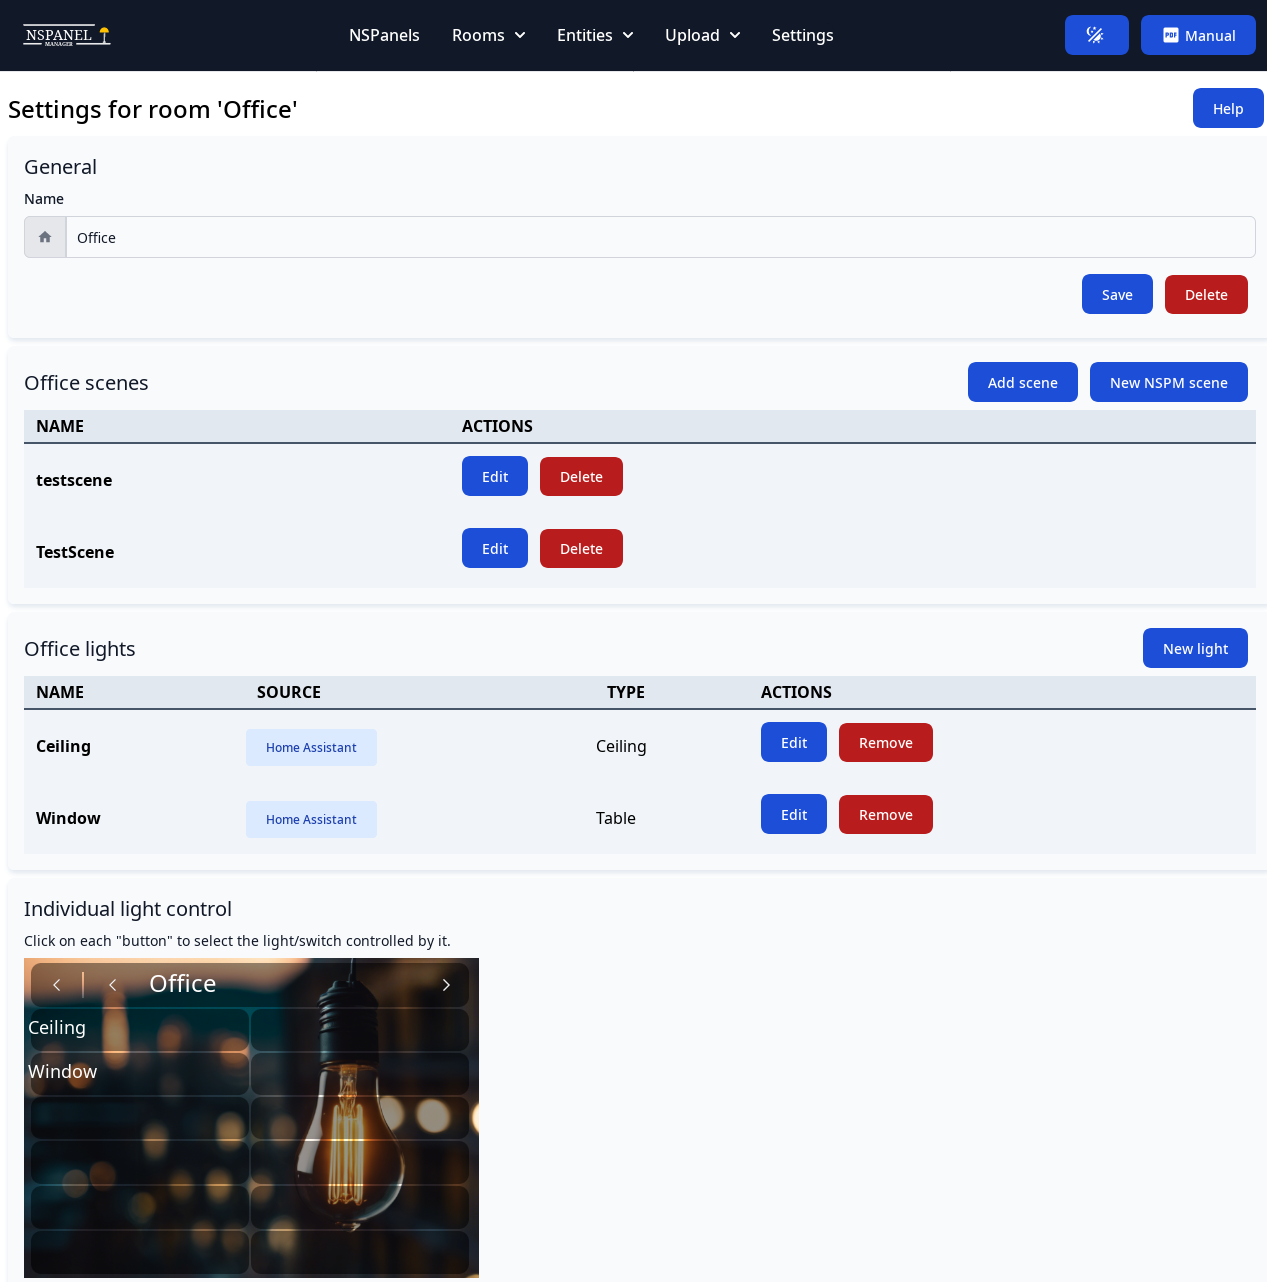
\includegraphics[width=\textwidth,height=\textheight,keepaspectratio]{room_page.png}
    \subsubsection{Scenes}
    At the moment, only NSPanel Manager scenes are available. They are easy enough to use. Simply create a scenes in the room page and they will be available in the "Scenes"-list for the room on all NSPanels.
    \\ To save a scene, on the NSPanel hold the save button for the scenes for 3 seconds to save all the states of lights \textbf{currently added to the room}.
    \\ To recall/activate a scene, on the NSPanel press the name of the scene and all the saved light states will be restored for that scene.
    \note{If a light was added after a scenes was saved, that light is not affected by that scenes until the scene is saved again.}
    \subsubsection{Lights}
    To add a new light, simply press the "Add new light"-button. When doing so, a list of all lights and switches gathered from Home Assistant and OpenHAB will be shown. Simply search or scroll to find the desired light and press it.
    \begin{figure}[H]
    \centering
    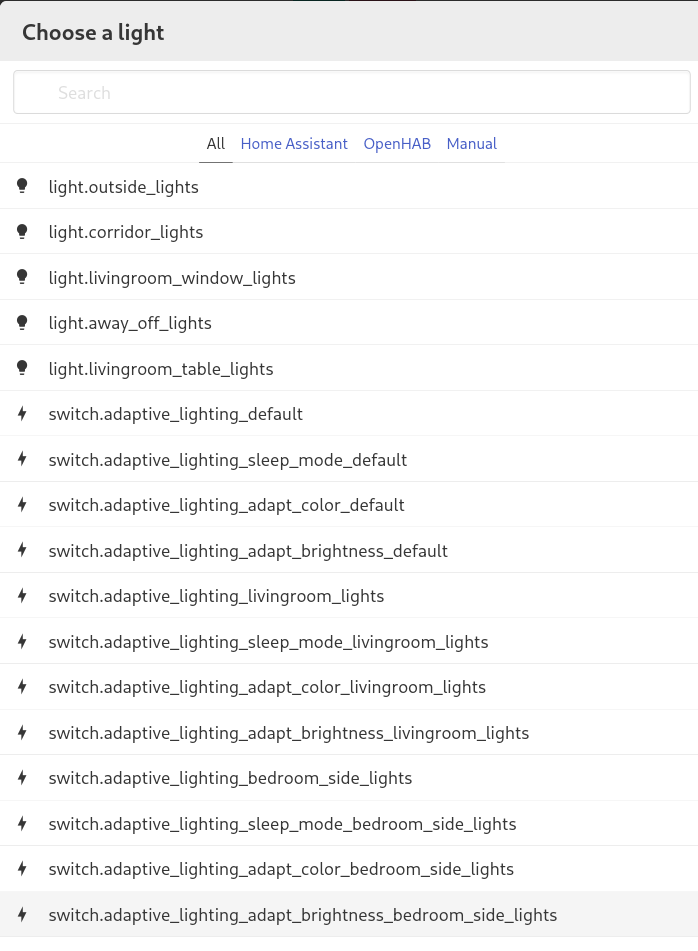
\includegraphics[scale=0.25]{add_new_light.png}
    \caption{Adding a new light to a room}%
    \end{figure}
    
    When done, a new screen will show up and depending on if the selected entity was from Home Assistant or OpenHAB.

    \begin{figure}[H]
    \centering
    \subfloat[\centering Home Assistant]{{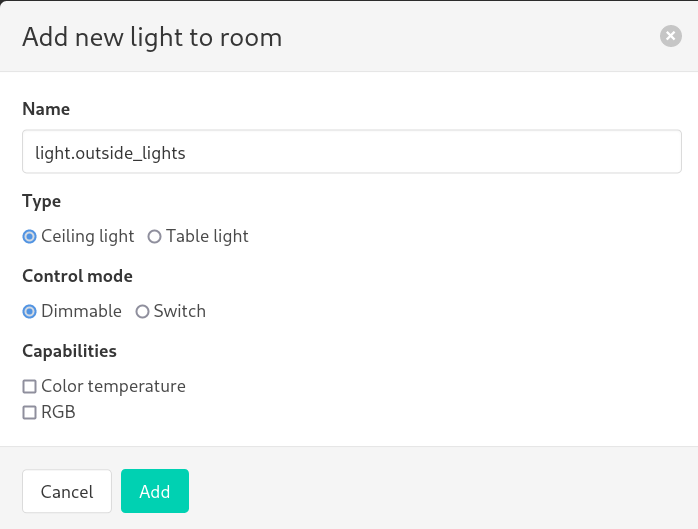
\includegraphics[width=5cm]{edit_new_light_ha.png} }}%
    \qquad
    \subfloat[\centering OpenHAB]{{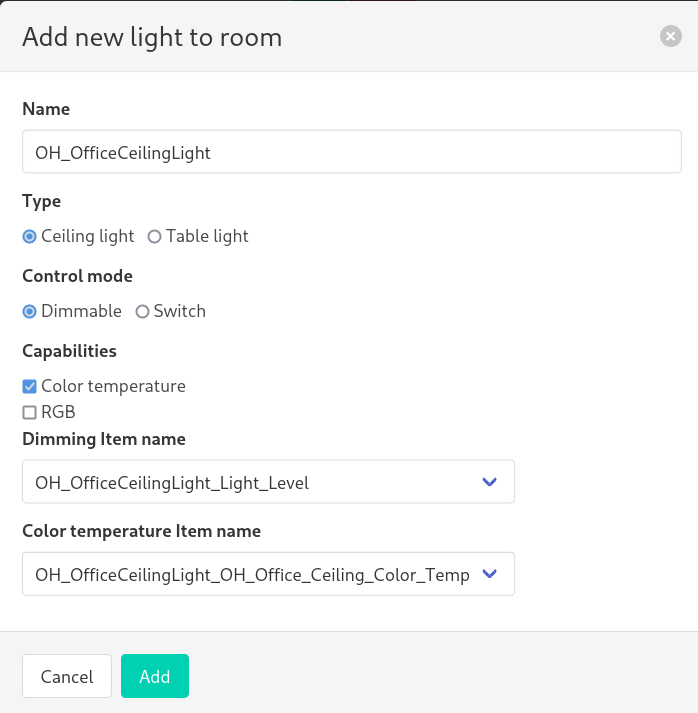
\includegraphics[width=5cm]{edit_new_light_openhab.png} }}%
    \caption{Add/Edit light}%
    \end{figure}
    
    When adding a Home Assistant entity, simply set a friendly name for it, select the type (Ceiling or Table light), select if it's a switch or dimmable light and what other capabilities it has.\\
    If you are adding an OpenHAB light or switch, things aren't as simple unfortunately. There is really no way around this but the user has to chose all the same settings as for Home Assistant but also has to select the appropriate OpenHAB items that corresponds to each capability of the light.

    \section{Panel functions}
    \subsection{Main page logic}
    The NSPanel main page might be a bit have some behavior that seems odd at first but the logic of it will be described here. The first page will affect entities in the selected room (if in room-mode) or all the configured lights (if in "All lights"-mode). The two left button for ceiling and table lights will always behave the same. Pressing a button that is "off" will turn on all the lights of that type. Pressing a button that is "on" will turn off all lights of that type. The sliders will always display an average value of all entities that will be affected of changes. There is really a few different scenarios:
    \subsubsection{One or more lights on}
    When changing the sliders, the changes will only be sent out to the lights currently on.
    If turning on a group of lights or individual lights they will be turned on to the current settings of the sliders. I.e. average dimming level and color temperature currently active.
    \subsubsection{No lights on}
    When changing the sliders, the changes will be sent out to all lights selected (depending on room or "all lights"-mode).
    \subsubsection{Lock mode}
    You can lock which light to affect by pressing and holding either the ceiling or table-lights button. This will enter a special mode where changes to the sliders will only affect the selected type of lights. By pressing the same button again you can exit the "special mode". The "special mode" will also time out after a few seconds.

    \clearpage
    \section{Logs}
    \label{sec:logs}
    While logs are normally sent over MQTT, any logs that are created before WiFi-connection are sent out on Serial. If you wish to see the logs going over MQTT, you can look at the topic \lstinline[language=bash]{nspanel/<panel name>/log}. If you wish to look at the logs going over serial, you can use programs like Putty. Connect to the NSPanel with the serial programmer as usual but \textbf{dont't} connect IO0 to GND. In Putty enter your serial port in the "Serial line" box and choose baud 115200. You should then be able to connect by pressing the "Open"-button. Example:
    \info{On Windows "/dev/ttyUSB0" will have to be replaced by something like "COM4". If using MacOS or Linux the port will be something similar to "/dev/ttyUSB0".}
    \begin{figure}[H]
    \centering
    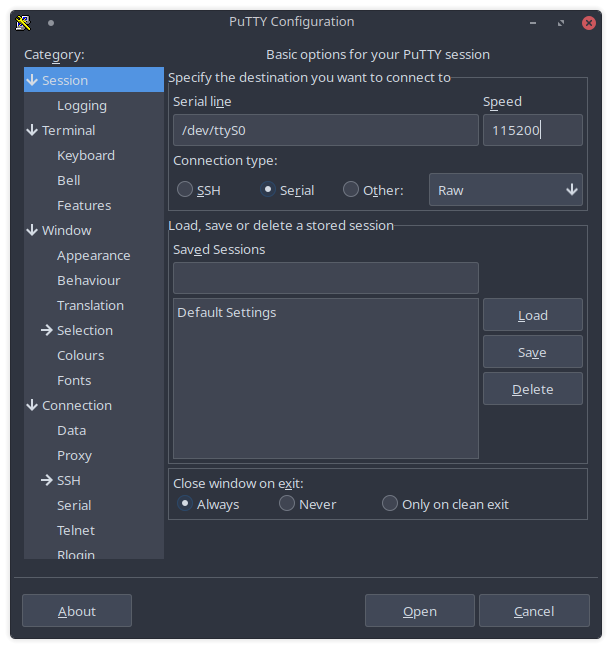
\includegraphics[scale=0.5]{putty_serial.png}
    \caption{Connecting to Serial with Putty}%
    \end{figure}

    \clearpage
    \section{Advanced setup}
    \label{sec:advanced_setup}
    \subsection{Manual Docker container setup}
    If you wish to manually build and setup the Docker container. To build the container, use the command \\ \lstinline[language=bash]{docker build -t nspanelmanager}. This will always be the same. To then start the container, the following command can be used:
    \begin{lstlisting}[language=bash]
    docker run --name nspanelmanager -v /etc/timezone:/etc/timezone:ro -v \
    "$(pwd)/web/nspanelmanager/db.sqlite3":"/usr/src/app/nspanelmanager/db.sqlite3" \
    -d -p 8000:8000 -p 8001:8001 nspanelmanager
    \end{lstlisting}
    If you wish to change the timezone, there are two options. Either, do as the command above, pass in the local machine /etc/timezone. This might not always work though as you'r server might be set to Etc/UTC then you can set the environment variable like this, for example: \lstinline[language=bash]{-E TZ=Europe/Stockholm} and remove the volume mapping for /etc/timezone.

    If you wish to change where the database is stored, replace "\$(pwd)/web/nspanelmanager/db.sqlite3" with where you wish your database to be stored on the local machine.


    \section{Functional information}
    \subsection{Data flow}

    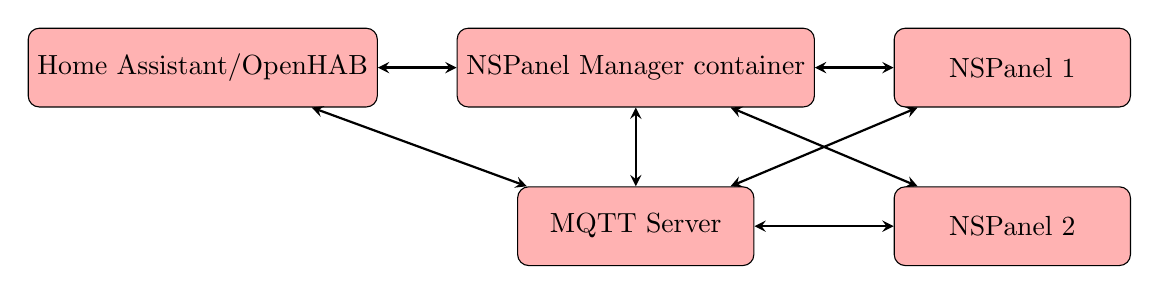
\begin{tikzpicture}
      \node (HAOpenHab) [startstop] {Home Assistant/OpenHAB};
      \node (NSPMcontainer) [startstop, right=of HAOpenHab] {NSPanel Manager container};
      \draw [doublearrow] (HAOpenHab) -- (NSPMcontainer);
      \node (MQTT) [startstop, below=of NSPMcontainer] {MQTT Server};
      \draw [doublearrow] (HAOpenHab) -- (MQTT);
      \draw [doublearrow] (NSPMcontainer) -- (MQTT);

      \node (panel1) [startstop, right=of NSPMcontainer] {NSPanel 1};
      \node (panel2) [startstop, below=of panel1] {NSPanel 2};
      \draw [doublearrow] (NSPMcontainer) -- (panel1);
      \draw [doublearrow] (NSPMcontainer) -- (panel2);
      \draw [doublearrow] (MQTT) -- (panel1);
      \draw [doublearrow] (MQTT) -- (panel2);

    \end{tikzpicture}
    

\end{document} % This is the end of the document
